\documentclass[10pt,letterpaper,xcolor=dvipsnames,handout]{beamer}

%\usepackage[colorlinks=true,linkcolor=blue]{hyperref}
\usepackage{amssymb,mathabx}
\usepackage{linguex}
\usepackage{verbatim,enumerate,multirow}
\usepackage{xcolor}
%\usepackage{floatflt}

\include{beamer-ru101f14}
\include{tikz-venn-diagrams}

\AtBeginSection[]
{
     \begin{frame}<beamer>
       \frametitle{Lecture plan}
       \tableofcontents[currentsection,currentsubsection]
   \end{frame}
}

\AtBeginSubsection[]
{
     \begin{frame}<beamer>
       \frametitle{Lecture plan}
       \tableofcontents[currentsection,currentsubsection]
   \end{frame}
}

\title{Categorical logic 3}
\subtitle{Syllogisms}
\author[Hoversten]{Erik Hoversten}
\institute[lrp-f14]{Logic, reason, and persuasion: fall 2014 \\ Rutgers University}
\date[10/08/2014]{October 8, 2014}

\begin{document}

\begin{frame}
\titlepage
\end{frame}

\section{From last time}

\frame{
  \frametitle{Standard form propositions}
  \framesubtitle{}
  
  \begin{block}{Schema}
    [Quantifier]+[(non-) subject term]+[copula]+[(non-) predicate term]
  \end{block}
  
  \begin{block}<2->{The complete language}
   \begin{itemize}
    \item All (non-)A are (non-)B
    \item No (non-)C are (non-)D
    \item Some (non-)E are (non-)F
    \item Some (non-)G are not (non-)H
   \end{itemize}
  \end{block}
}

\frame{
  \frametitle{Direct inferences}
  \framesubtitle{}
  
    \begin{block}{What are the?}
   \begin{itemize}
    \item Direct inferences are one premise arguments.
    \item The conclusion is meant to be an equivalent restatement of the premise.
   \end{itemize}
  \end{block}
  
    \begin{block}<2->{Assessing their validity}
   \begin{itemize}
    \item There are two methods for assessing the validity of a direct inference.
    \item Method 1: Contradictory relation plus Venn diagrams
    \item Method 2: Other semantics relations plus the Square of Opposition
   \end{itemize}
  \end{block}
}

\frame{
  \frametitle{Assessing validity}
  \framesubtitle{Method 1}
  
  \begin{block}{Get into standard form}
   \begin{itemize}
    \item The first step is to get each of the propositions in the inference into \textbf{standard form}.
    \item We do this by translating propositions that start with ``It is false that...'' into true propositions, using the contradictory relation on the square of opposition.
   \end{itemize}
  \end{block}
  
  \begin{block}<2->{Compare the Venn diagrams}
  Construct the Venn diagram for both propositions in standard form, and compare the premise diagram to that of the conclusion.
   \begin{description}
    \item[Valid=] the conclusion says no more than the premise.
    \item[Invalid=] the conclusion says more than the premise, \textbf{or} it conflicts with the premise.
    \item[Conditionally valid=] the inference is valid, but there is a \tikz\node [draw, rounded corners] {x}; in one of the diagrams.
   \end{description}
  \end{block}
}

\frame{
  \frametitle{Assessing validity}
  \framesubtitle{Method 2}
  
  \begin{block}{Other semantics relations}
   \begin{itemize}
    \item We used the square of opposition to define other semantic relations between propositions.
    \item Contrary, subcontrary, and subalternation
    \item If the two propositions of the inference stand in one of these relations, then we can use the purported truth value of one of them to infer the truth value of the other.
   \end{itemize}
  \end{block}
   
   \begin{block}<2->{Example}
   \begin{enumerate}
    \item It is false that some A are B.
    \item $\therefore$, Some A are not B.
   \end{enumerate}
  \end{block}
  
    \uncover<3->{These propositions stand in the relation of \textit{subcontrary}. For subcontraries, it is impossible for both of them to be false.  So, if the first proposition is false, then it is indeed the case that the second one must be true.}
}

\section{Categorical syllogisms}

\frame{
\frametitle{Categorical syllogisms}
\framesubtitle{Definition}

\begin{block}{Two premise arguments}
 \begin{itemize}
  \item Conclusion
  \begin{itemize}
   \item Predicate = \textbf{major term}
   \item Subject = \textbf{minor term}
  \end{itemize}
  \item Major premise (contains the major term and a middle term)
  \item Minor premse (contains the minor term and the middle term)
 \end{itemize}
 \end{block}
 
   \begin{block}<2->{Form}
   \begin{enumerate}
    \item $\,$[Quant]+[Major/middle term]+[copula]+[Middle/major term]
    \item $\,$[Quant]+[Minor/middle term]+[copula]+[Middle/minor term]
    \item $\,$[Quant]+[Minor term]+[copula]+[Major term]
   \end{enumerate}
  \end{block}
}

\frame{
  \frametitle{Standard form}
  \framesubtitle{}
  
  \begin{block}{A categorical syllogism is in standard form if...}
   \begin{enumerate}
    \item All three statements are standard form categorical propositions.
    \item The major, minor, and middle terms each appear twice.
    \item The two occurrences of each term are identical.
    \item Each term is used in the same sense throughout the argument.
    \item The major premise is listed first, the minor premise second, and the comclusion third.
   \end{enumerate}

  \end{block}
  
  \begin{block}<2->{Example}
   \begin{enumerate}
    \item All flying things have wings.   
    \item Some birds are flying things.
    \item $\therefore$, some birds have wings.
   \end{enumerate}

  \end{block}

}

\section{Representing syllogisms}

\subsection{Mood and figure}

\frame{
  \frametitle{Mood}
  \framesubtitle{What is it?}
  
    \begin{block}{Mood}
   \begin{itemize}
    \item The kinds of proposition that make up the syllogism constitute its \textbf{mood}
    \item We use letters to represent the kinds of propositions.
    \begin{description}
     \item [A] = All A are B
     \item [E] = No A are B 
     \item [I] = Some A are B 
     \item [O] = Some A are not B 
    \end{description}
    \item We represent the mood of the syllogism by writing the letters corresponding to each of its propositions in order.
   \end{itemize}
  \end{block}
  \vspace{.5cm}
\uncover<2->{
\begin{center}
\begin{tabular}{llll}
 1. & Some B are not C. & & \\
 2. & All A are B. & $\rightarrow$ & \textbf{OAE} \\
 3. & $\therefore$, No A are C. & & \\
\end{tabular}
\end{center}
}
}

\frame{
\frametitle{Figure}
\framesubtitle{What is it?}

\begin{block}{Figure}
 \begin{itemize}
  \item The relative positions of the terms in the propositions determines the figure of the argument.
  \item S = subject term, P = predicate term, \textcolor{red}{M} = middle term.
 \end{itemize}
\end{block}

\uncover<2->{
\begin{columns}
 \column{.5\textwidth}
 \begin{center}
  \underline{Figure 1} \\
  \textcolor{red}{M} \hspace{1cm} P \\
  \underline{S \hspace{1cm} \textcolor{red}{M}} \\
  S \hspace{1cm} P \\
  \vspace{.75cm}
    \underline{Figure 3} \\
  \textcolor{red}{M} \hspace{1cm} P \\
  \underline{\textcolor{red}{M} \hspace{1cm} S} \\
  S \hspace{1cm} P \\
  \end{center}
 \column{.5\textwidth}
 \begin{center}
   \underline{Figure 2} \\
  P \hspace{1cm} \textcolor{red}{M} \\
  \underline{S \hspace{1cm} \textcolor{red}{M}} \\
  S \hspace{1cm} P \\
  \vspace{.75cm}
    \underline{Figure 4} \\
  P \hspace{1cm} \textcolor{red}{M} \\
  \underline{\textcolor{red}{M} \hspace{1cm} S} \\
  S \hspace{1cm} P \\
  \end{center}
\end{columns}
}
}

\frame{
\frametitle{Validity tables}
\framesubtitle{}

\begin{block}{Complete specification}
 \begin{itemize}
  \item With mood and form in hand, we can specify simply every possible categorical syllogism. (There are 64 of them.)
  \item And we can rely on the time that others have put in testing each of the forms for validity.
  \item The result is compiled in the table below.
 \end{itemize}
 \end{block}
 
\uncover<2->{
 \begin{center}
 \begin{tabular}{c|c|c|c}
  \textbf{Figure 1} & \textbf{Figure 2} & \textbf{Figure 3} & \textbf{Figure 4} \\ \hline
  AAA & EAE & IAI & AEE \\
  EAE & AEE & AII & IAI \\
  AII & EIO & OAO & EIO \\
  EIO & AOO & EIO & \\
 \end{tabular}
 \end{center}
}
}

\subsection{Venn diagrams}

\frame{
\frametitle{Arguments in Venn diagrams}
\framesubtitle{}

\begin{block}{All true together}
 \begin{itemize}
  \item Valid arguments are supposed to be such that the conclusion is contained within the premises.
  \item So, if a syllogism is valid, we should be able to represent all the propositions of the argument within one, unified diagram.
  \item The only thing that changes is that we have an extra term hanging around (the middle term), so we need to add in an extra circle to represent that class.
 \end{itemize}

\end{block}

}

\frame{
  \frametitle{Representing categorical syllogisms}
  \framesubtitle{Venn diagrams}
  
  \begin{center}
   \begin{tikzpicture}
    \begin{scope}[fill opacity=0.5]
     \fill[red] \firstcircle;
     \fill[blue] \secondcircle;
     \fill[green] \thirdcircle;
    \end{scope}
    \syllbox{A}{B}{C}
   \end{tikzpicture}
  \end{center}  
}

\frame{
\frametitle{Example \#1}
\framesubtitle{EAE-2}

\begin{columns}
 \column{.4\textwidth}
 \begin{enumerate}
  \item \alert{No P are M}
  \item All S are M
  \item $\therefore$, No S are P
 \end{enumerate}

 \column{.6\textwidth}
 \begin{tikzpicture}
  \filltopright{red}
  \syllbox{S}{P}{M}
 \end{tikzpicture}
 
\end{columns}
}

\frame{
\frametitle{Example \#1}
\framesubtitle{EAE-2}

\begin{columns}
 \column{.4\textwidth}
 \begin{enumerate}
  \item No P are M
  \item \alert{All S are M}
  \item $\therefore$, No S are P
 \end{enumerate}
 
 \column{.6\textwidth}
 \begin{tikzpicture}
 \filltopright{red}
 \begin{scope}[even odd rule, fill opacity=0.5]
    \clip \thirdcircle (-1,-1) rectangle (1,1);
    \fill[blue] \firstcircle;
  \end{scope}
  \syllbox{S}{P}{M}
 \end{tikzpicture}
 
\end{columns}
}

\frame{
\frametitle{Example \#1}
\framesubtitle{EAE-2}

\begin{columns}
 \column{.4\textwidth}
 \begin{enumerate}
  \item No P are M
  \item All S are M
  \item \alert{$\therefore$, No S are P}
 \end{enumerate}
 
 Valid
 
 \column{.6\textwidth}
 \begin{tikzpicture}
  \filltopright{red}
  \begin{scope}[even odd rule, fill opacity=0.5]
    \clip \thirdcircle (-1,-1) rectangle (1,1);
    \fill[blue] \firstcircle;
  \end{scope}
  \syllbox{S}{P}{M}
 \end{tikzpicture}
 
\end{columns}
}

\frame{
\frametitle{Example \#2}
\framesubtitle{IAI-4}

\begin{columns}
 \column{.4\textwidth}
 \begin{enumerate}
  \item Some P are M
  \item \alert{All M are S}
  \item $\therefore$, Some S are P
 \end{enumerate}
 
 \column{.6\textwidth}
 \begin{tikzpicture}
  \filltopfirst
  \syllbox{S}{P}{M}
 \end{tikzpicture}
 
\end{columns}
}

\frame{
\frametitle{Example \#2}
\framesubtitle{IAI-4}

\begin{columns}
 \column{.4\textwidth}
 \begin{enumerate}
  \item \alert{Some P are M}
  \item All M are S
  \item $\therefore$, Some S are P
 \end{enumerate}
 
 \column{.6\textwidth}
 \begin{tikzpicture}
  \filltopfirst
  \xtopmid
  \syllbox{S}{P}{M}
 \end{tikzpicture}
 
\end{columns}
}

\frame{
\frametitle{Example \#2}
\framesubtitle{IAI-4}

\begin{columns}
 \column{.4\textwidth}
 \begin{enumerate}
  \item Some P are M
  \item All M are S
  \item \alert{$\therefore$, Some S are P}
 \end{enumerate}
 
 Valid
 
 \column{.6\textwidth}
 \begin{tikzpicture}
  \filltopfirst
  \xtopmid
  \syllbox{S}{P}{M}
 \end{tikzpicture}
 
\end{columns}
}

\frame{
\frametitle{Example \#3}
\framesubtitle{AEE-1}

\begin{columns}
 \column{.4\textwidth}
 \begin{enumerate}
  \item \alert{All M are P}
  \item No S are M
  \item $\therefore$, No S are P
 \end{enumerate}
 
 \column{.6\textwidth}
 \begin{tikzpicture}
  \filltopsecond
  \syllbox{S}{P}{M}
 \end{tikzpicture}
 
\end{columns}
}

\frame{
\frametitle{Example \#3}
\framesubtitle{AEE-1}

\begin{columns}
 \column{.4\textwidth}
 \begin{enumerate}
  \item All M are P
  \item \alert{No S are M}
  \item $\therefore$, No S are P
 \end{enumerate}
 
 \column{.6\textwidth}
 \begin{tikzpicture}
  \filltopsecond
  \filltopleft{blue}
  \syllbox{S}{P}{M}
 \end{tikzpicture}
 
\end{columns}
}

\frame{
\frametitle{Example \#3}
\framesubtitle{AEE-1}

\begin{columns}
 \column{.4\textwidth}
 \begin{enumerate}
  \item All M are P
  \item No S are M
  \item \alert{$\therefore$, No S are P}
 \end{enumerate}
 
 Invalid
 
 \column{.6\textwidth}
 \begin{tikzpicture}
  \filltopsecond
  \filltopleft{blue}
  \fillmiddle
  \syllbox{S}{P}{M}
 \end{tikzpicture}
 
\end{columns}
}

\frame{
\frametitle{Example \#4}
\framesubtitle{OIO-1}

\begin{columns}
 \column{.4\textwidth}
 \begin{enumerate}
  \item \alert{Some M are not P}
  \item Some S are M
  \item $\therefore$, Some S are not P
 \end{enumerate}
 
 \column{.6\textwidth}
 
\begin{tikzpicture}
   \draw (70:1cm) node [text=red] {\textbf{X}};
  \syllbox{S}{P}{M}
 \end{tikzpicture}
 
\end{columns}
}

\frame{
\frametitle{Example \#4}
\framesubtitle{OIO-1}

\begin{columns}
 \column{.4\textwidth}
 \begin{enumerate}
  \item Some M are not P
  \item \alert{Some S are M}
  \item $\therefore$, Some S are not P
 \end{enumerate}
 
 \column{.6\textwidth}
 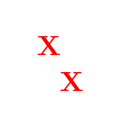
\begin{tikzpicture}
    \draw (70:1cm) node [text=red] {\textbf{X}};
    \draw (38:.8cm) node [text=red] {\textbf{X}};
  \syllbox{S}{P}{M}
 \end{tikzpicture}
 
\end{columns}
}

\frame{
\frametitle{Example \#4}
\framesubtitle{OIO-1}

\begin{columns}
 \column{.4\textwidth}
 \begin{enumerate}
  \item Some M are not P
  \item Some S are M
  \item \alert{$\therefore$, Some S are not P}
 \end{enumerate}
 
 Invalid: Premises allow for the conclusion to be either true or false.
 
 \column{.6\textwidth}
 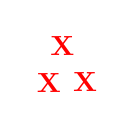
\begin{tikzpicture}
  \draw (70:1cm) node [text=red] {\textbf{X}};
  \draw (38:.8cm) node [text=red] {\textbf{X}};
  \draw (70:.5cm) node [text=red] {\textbf{X}};
  \syllbox{S}{P}{M}
 \end{tikzpicture}
 
\end{columns}
}

\frame{
\frametitle{Bonus assignment on Informal fallacies}
\framesubtitle{Completely optional}

\begin{block}{Recognizing fallacies}
 \begin{itemize}
  \item In the book, Ch.3, section 4 exercises, pp. 180-181
  \item There is a passage called ``Personal Paper Mill''
  \item This passage contains a number of fallacies that we went over in class.
  \item If you can locate and identify some of these fallacies, you can get some bonus points toward your class grade.
  \item 1 point for each fallacy, up to 5 points total.
  \item You may submit 6 fallacies, but can get a maximum of 5 points.
  \item You should write out the sentences where the fallacy occurs and label it with the appropriate fallacy name.
  \item Assignment must be submitted to me by Monday October 20th (miderm exam day).
 \end{itemize}

\end{block}

}
\end{document}